% \textbf{\underline{OZ 8 - $ LC $- en $ RLC $-circuits - Oefening 2:}}
% \vspace{0.5cm}

% De schakelaar in figuur 8.1 wordt gedurende lange tijd in punt $ a $ gehouden. Op $ t = 0 $ wordt de schakelaar naar punt $ b $ geschoven. Bepaal

% \begin{enumerate}[(a)]
%     \item de frequentie van de oscillatie in het $ LC $-circuit,
%     \item de maximum lading op de condensator,
%     \item de maximum stroom door de spoel,
%     \item en de totale energie in het circuit op $ t = 3,00 $ s.
% \end{enumerate}

% \begin{figure}[H]
%     \centering
%     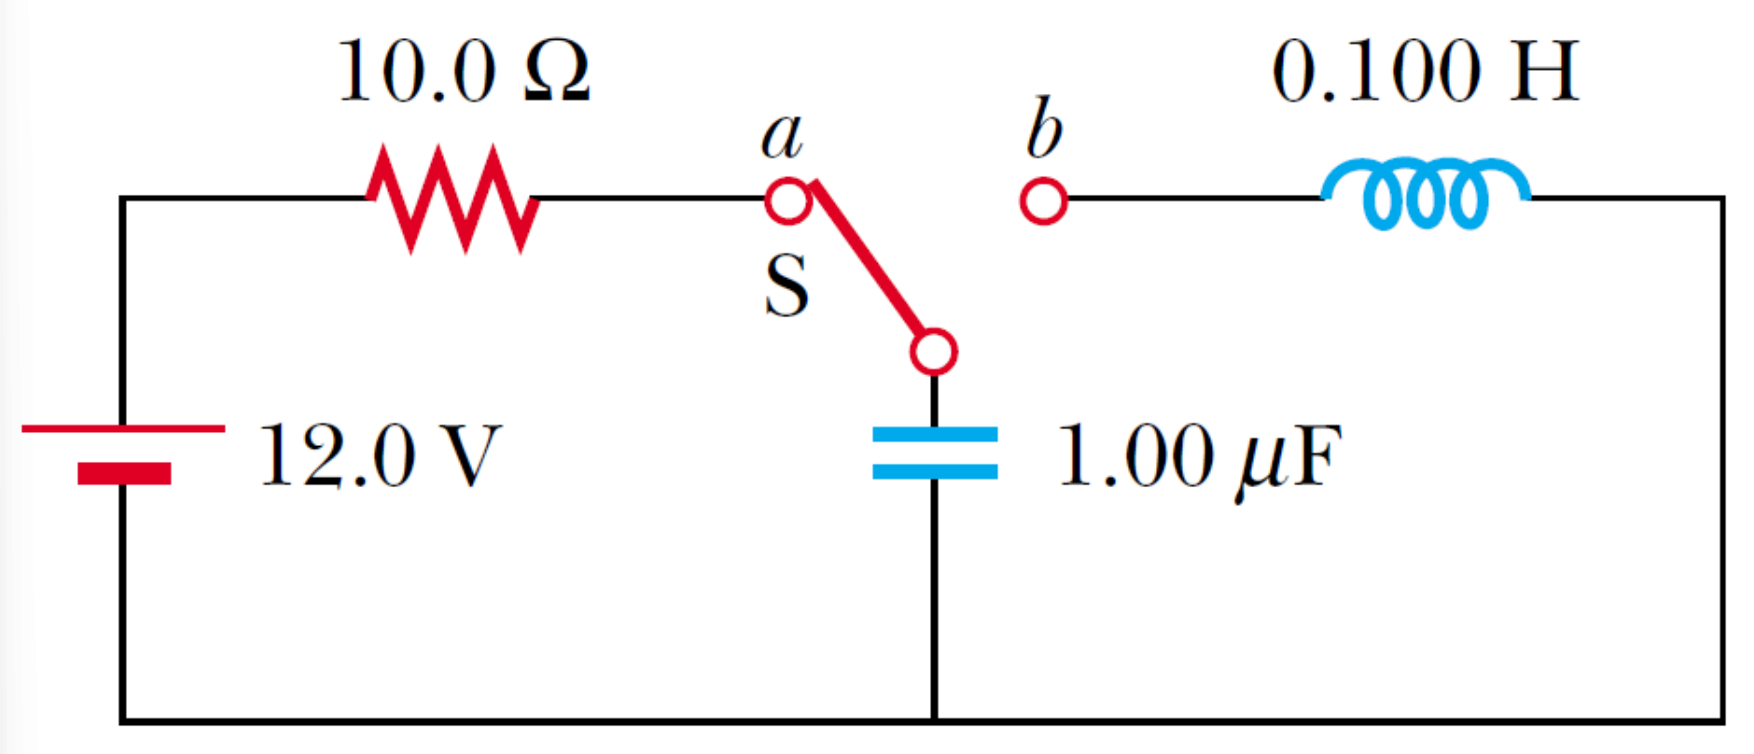
\includegraphics[width=6cm]{oz08/resources/oef-2-opgave.png}
    
%     \textbf{Figuur 8.1}
% \end{figure}

% \begin{description}[labelwidth=1.5cm, leftmargin=!]
%     \item[Geg. :]   $ \varepsilon = 12,0 $ V; $ R = 10,0 \ \Omega $; $ C = 1,00 \ \mu $F; $ L = 0,100 $ H;
% \end{description}

% \begin{enumerate}[(a)]
%     \item 
%         \begin{description}[labelwidth=1.5cm, leftmargin=!]
%             \item[Gevr. :]  $ f $;
%             \item[Opl. :]   $ I \cdot X_C = I \cdot X_L $
                            
%                             \hspace{-0.57cm} $ \Leftrightarrow
%                             X_C = X_L $
                            
%                             \hspace{-0.57cm} $ \Leftrightarrow
%                             \dfrac{1}{\omega C} = \omega L $
                            
%                             \hspace{-0.57cm} $ \Leftrightarrow
%                             \omega = \sqrt{\dfrac{1}{L C}} = \dfrac{1}{\sqrt{L C}} $
                            
%                             \vspace{0.5cm}
                            
%                             $ f = \dfrac{\omega}{2 \pi} 
%                             = \dfrac{1}{2 \pi \sqrt{L C}} 
%                             = \dfrac{1}{2 \pi \sqrt{0,100 \cdot 1,00 \cdot 10^{-6}}} 
%                             = 503,292121 $ Hz $
%                             \approx 503 $ Hz
%         \end{description}
%     \item
%         \begin{description}[labelwidth=1.5cm, leftmargin=!]
%             \item[Gevr. :]  $ Q_{max} $;
%             \item[Opl. :]   $ Q = Q_{max} \to I = 0 $ A
            
%                             $ \varepsilon = I \cdot R + V_C = 0 \cdot R + V_C = V_C $
                            
%                             \hspace{-0.57cm} $ \Leftrightarrow 
%                             V_C = \varepsilon $
                            
%                             $ Q_{max} = C \cdot V_C = C \cdot \varepsilon 
%                             = 1,00 \cdot 10^{-6} \cdot 12,0 
%                             = 0,000012 $ C $ 
%                             = 12,0 \ \mu$C 
%         \end{description}
%     \item
%         \begin{description}[labelwidth=1.5cm, leftmargin=!]
%             \item[Gevr. :]  $ I_{max} $;
%             \item[Opl. :]   $ V_C = I \cdot X_C $
            
%                             \hspace{-0.57cm} $ \Leftrightarrow
%                             \dfrac{Q_{max}}{C} = I_{max} \cdot \dfrac{1}{\omega C} $
            
%                             \hspace{-0.57cm} $ \Leftrightarrow
%                             I_{max} = \omega Q_{max} 
%                             = \dfrac{Q_{max}}{\sqrt{L C}} 
%                             = \dfrac{0,000012}{\sqrt{0,100 \cdot 1,00 \cdot 10^{-6}}} 
%                             = 0,037947332 $ A $ 
%                             \approx 37,9 $ mA
%         \end{description}
%     \item
%         \begin{description}[labelwidth=1.5cm, leftmargin=!]
%             \item[Geg. :]   $ t = 3,00 $ s;
%             \item[Gevr. :]  $ U_{tot} $;
%             \item[Opl. :]   $ V_C = -V_L = -L \dfrac{dI}{dt} $
                            
%                             \hspace{-0.57cm} $ \Rightarrow 
%                             \dfrac{dV_C}{dt} = -L \dfrac{d^2I}{dt^2} $
                            
%                             \vspace{0.5cm}
                            
%                             $ I = C \dfrac{dV_C}{dt} = -LC \dfrac{d^2I}{dt^2} $
                            
%                             \hspace{-0.57cm} $ \Leftrightarrow 
%                             \dfrac{d^2I}{dt^2} + \dfrac{1}{LC} I = 0 $
                            
%                             \hspace{-0.57cm} $ \Leftrightarrow 
%                             \dfrac{d^2I}{dt^2} + \omega^2 I = 0 $
                            
%                             \vspace{0.5cm}
                            
%                             \hspace{-0.57cm} $ \Rightarrow 
%                             I(t) = c_1 \sin{\left( \omega t \right)} + c_2 \cos{\left( \omega t \right)} $
                            
%                             \vspace{0.5cm}
                            
%                             $ I(t = 0) = 0 $
                            
%                             \hspace{-0.57cm} $ \Leftrightarrow 
%                             c_1 \sin{\left( \omega \cdot 0 \right)} + c_2 \cos{\left( \omega \cdot 0 \right)} = 0 $
                            
%                             \hspace{-0.57cm} $ \Leftrightarrow 
%                             c_1 = 0 $
                            
%                             \vspace{0.5cm}
                            
%                             \hspace{-0.57cm} $ \Rightarrow 
%                             I(t) = c_2 \cos{\left( \omega t \right)} $
                            
%                             \hspace{-0.57cm} $ \Rightarrow
%                             \dfrac{dI}{dt} = - c_2 \omega \sin{\left( \omega t \right)} $
                            
%                             \vspace{0.5cm}
                            
%                             $ V_{C}(t) = -L \dfrac{dI}{dt} 
%                             = L c_2 \omega \sin{\left( \omega t \right)}
%                             = c_2 \sqrt{\dfrac{L}{C}} \sin{\left( \omega t \right)} $
                            
%                             \vspace{0.5cm}
                            
%                             $ V_{C}(t = 0) = V_{C,max} $
                            
%                             \hspace{-0.57cm} $ \Leftrightarrow
%                             c_2 \sqrt{\dfrac{L}{C}} \sin{\left( \omega \cdot 0 \right)} = \varepsilon $
                            
%                             \hspace{-0.57cm} $ \Leftrightarrow
%                             c_2 \sqrt{\dfrac{L}{C}} = \varepsilon $
                            
%                             \hspace{-0.57cm} $ \Leftrightarrow
%                             c_2 = \varepsilon \sqrt{\dfrac{C}{L}} $
                            
%                             \vspace{0.5cm}
                            
%                             \hspace{-0.57cm} $ \Rightarrow 
%                             I(t) = \varepsilon \sqrt{\dfrac{C}{L}} \cos{\left( \omega t \right)} 
%                             = \varepsilon \sqrt{\dfrac{C}{L}} \cos{\left( \dfrac{t}{\sqrt{L C}} \right)} $
                            
%                             \vspace{0.5cm}
                            
%                             \hspace{-0.57cm} $ \Rightarrow 
%                             V_C(t) = \varepsilon \sqrt{\dfrac{C}{L}} \sqrt{\dfrac{L}{C}} \sin{\left( \omega t \right)}
%                             = \varepsilon \sin{\left( \dfrac{t}{\sqrt{L C}} \right)} $
                            
%                             \vspace{0.5cm}
                            
%                             $ I(t = 3,00) = \varepsilon \sqrt{\dfrac{C}{L}} \cos{\left( \dfrac{3,00}{\sqrt{L C}} \right)} $
                            
%                             \hspace{1.7cm} $ = 12,0 \sqrt{\dfrac{1,00 \cdot 10^{-6}}{0,100}} \cos{\left( \dfrac{3,00}{\sqrt{0,100 \cdot 1,00 \cdot 10^{-6}}} \right)} $
                            
%                             \hspace{1.7cm} $ = 0,027061647 $ A
                            
%                             \vspace{0.5cm}
                            
%                             $ V_C(t = 3,00) = \varepsilon \sin{\left( \dfrac{3,00}{\sqrt{L C}} \right)} $
                            
%                             \hspace{1.95cm} $ 
%                             = 12,0 \sin{\left( \dfrac{3,00}{\sqrt{0,100 \cdot 1,00 \cdot 10^{-6}}} \right)} $
                            
%                             \hspace{1.95cm} $ 
%                             = -8,412296068 $ V
                            
%                             \vspace{0.5cm}
                            
%                             $ U_L = \dfrac{1}{2} L I^2 = \dfrac{1}{2} \cdot 0,100 \cdot 0,027061647^2 
%                             = 0,000036617 $ J
                            
%                             $ U_C = \dfrac{1}{2} C V_C^2 = \dfrac{1}{2} \cdot 1,00 \cdot 10^{-6} \cdot \left( -8,412296068 \right)^2 
%                             = 0,000035383 $ J
                            
%                             $ U_{tot} = U_L + U_C = 0,000036617 + 0,000035383 
%                             = 0,000072 $ J $ 
%                             = 72,0 \ \mu$J
%         \end{description}
% \end{enumerate}

% \vspace{1cm}